
\documentclass[12pt]{article}

\usepackage{amsfonts}
\usepackage{amsmath}
\usepackage{amssymb}
\usepackage{cite}
\usepackage{enumerate}
\usepackage{fancyhdr}
\usepackage[headheight=1in,margin=1.25in]{geometry}
\usepackage[colorlinks=true,linkcolor=blue]{hyperref}
\usepackage{mathtools}
\usepackage{setspace}

\usepackage{tikz}

\newcommand{\N}{\ensuremath{\mathbb{N}}}
\newcommand{\Z}{\ensuremath{\mathbb{Z}}}
\newcommand{\Q}{\ensuremath{\mathbb{Q}}}
\newcommand{\R}{\ensuremath{\mathbb{R}}}
\newcommand{\C}{\ensuremath{\mathbb{C}}}

\newcommand{\e}{\ensuremath{\varepsilon}}
\renewcommand{\d}{\ensuremath{\delta}}

\newcommand{\angleb}[1]{\left\langle#1\right\rangle}
\newcommand{\braceb}[1]{\left\{#1\right\}}
\newcommand{\bracketb}[1]{\left[#1\right]}
\newcommand{\parenb}[1]{\left(#1\right)}
\newcommand{\vertb}[1]{\left\vert#1\right\vert}
\newcommand{\dvertb}[1]{\left\Vert#1\right\Vert}

\DeclarePairedDelimiter\floor{\lfloor}{\rfloor}
\DeclarePairedDelimiter\ceil{\lceil}{\rceil}

\newcommand{\comp}{\complement}
\newcommand{\sdiff}{\setminus}

\newcommand{\proof}{\textit{Proof: }}
\newcommand{\partialdone}{\ensuremath{\strut\hfill\blacktriangle}}
\newcommand{\done}{\ensuremath{\strut\hfill\blacksquare}}

\newcommand{\mc}[1]{\ensuremath{\mathcal{#1}}}

\renewcommand{\t}[1]{\text{ #1 }}
\newcommand{\impl}{\ensuremath{\implies}}
\newcommand{\sectionskip}{\vspace{0.15in}}
\newcommand{\tri}{\triangle}

\begin{document}

\pagestyle{fancy}
\fancyhead[L]{Ahlfors}
\fancyhead[C]{Complex Analysis}
\fancyhead[R]{Chapter 1}

\setlength{\parindent}{0in}
\setlength{\parskip}{0.1in}
\setstretch{1}

\section*{Section 1.1}

\textbf{1)} Represent the following values in the form \( a + bi \), where
\( a, b \in \R\).
\[
	(1 + 2i)^3, \quad
	\frac{5}{-3 + 4i}, \quad
	\parenb{ \frac{2 + i}{3 - 2i} }^2, \quad
	(1 + i)^n + (1 - i)^n
\]

\textbf{Solution:}
\[ (1 + 2i)^3 = (-3 + 4i)(1 + 2i) = \boxed{-11 - 2i} \]
\[
	\frac{5}{-3 + 4i} =
	\frac{5}{-3 + 4i} \cdot \frac{-3 - 4i}{-3 - 4i} =
	\frac{-15 - 20i}{25} =
	\boxed{-\frac{3}{5} - \frac{4}{5}i}
\]
\[
	\parenb{\frac{2 + i}{3 - 2i}}^2 =
	\frac{2 + i}{3 - 2i} \cdot \frac{2 + i}{3 - 2i} =
	\frac{3 + 4i}{5 - 12i} =
	\frac{3 + 4i}{5 - 12i} \cdot \frac{5 + 12i}{5 + 12i} =
	\frac{-33 + 56i}{169}
\]
\[ = \boxed{-\frac{33}{169} + \frac{56}{169}i} \]

Using the binomial theorem, we see that
\[
	(1 + i)^n + (1 - i)^n
	= \sum_{k = 0}^n \binom{n}{k}i^k + \sum_{k = 0}^n \binom{n}{k}(-i)^k
	= \sum_{k = 0}^n \binom{n}{k} \bracketb{i^k + (-i)^k}.
\]
Since \( i = (-i)^3 \) and \( -i = i^3 \), we have that
\( i^k + (-i)^k = 0 \) for odd \( k \), thus it suffices to consider the even
terms of the sum.
Additionally, since \( i^2 = (-i)^2 = -1 \) and \( i^4 = (-i)^4 = 1 \), we have
\( i^k + (-i)^k = 2(-1)^k \) for even \( k \).
This gives us
\[
	(1 + i)^n + (1 - i)^n
	= \boxed{\sum_{k = 0}^{\floor{n/2}} \binom{n}{2k} 2(-1)^{2k}}
\]
and thus we obtain a real number for all values of \( n \).

\textbf{2)} Letting \( z = a + bi \) for \( a,b \in \R \), find the real and
imaginary parts for the following complex numbers:
\[
	z^4, \quad
	\frac{1}{z}, \quad
	\frac{z - 1}{z + 1}, \quad
	\frac{1}{z^2}
\]

\textbf{Solution:}
\[
	z^4 = (a + bi)^4 = (a + bi)^2 (a + bi)^2 = (a^2 + 2abi - b^2)^2
\]
\[
	= \boxed{a^4 - 6a^2b^2 + b^4 + (4a^3b  - 4ab^3)i}
\]
\[
	\frac{1}{z} = \frac{1}{a + bi} \cdot \frac{a - bi}{a - bi}
	= \frac{a - bi}{a^2 + b^2}
	= \boxed{\frac{a}{a^2 + b^2} - \frac{b}{a^2 + b^2}i}
\]
\[
	\frac{z - 1}{z + 1} = \frac{a - 1 + bi}{a + 1 + bi}
	\cdot \frac{a + 1 - bi}{a + 1 - bi}
	= \frac{(a - 1 + bi)(a + 1 - bi)}{(a + 1)^2 + b^2}
	= \frac{a^2 + b^2 - 1 + 2bi}{(a + 1)^2 + b^2}
\]
\[
	= \boxed{
		\frac{a^2 + b^2 - 1}{(a + 1)^2 + b^2}
		+ \frac{2b}{(a + 1)^2 + b^2}i
	}
\]
\[
	\frac{1}{z^2} = \frac{1}{(a + bi)^2} = \frac{1}{a^2 - b^2 + 2abi}
	= \frac{1}{a^2 - b^2 + 2abi}
	\cdot \frac{a^2 - b^2 - 2abi}{a^2 - b^2 - 2abi}
\]
\[
	= \frac{a^2 - b^2 - 2abi}{a^4 + 2a^2b^2 + b^4}
	= \boxed{
		\frac{a^2 - b^2}{(a^2 + b^2)^2} - \frac{2ab}{(a^2 + b^2)^2}i
	}
\]

\textbf{3)} We have that
\[
	\parenb{\frac{-1 \pm i\sqrt{3}}{2}}^3
	= \parenb{\frac{\pm 1 \pm i\sqrt{3}}{2}}^6
	= 1
\]
for all combinations of \( + \) and \( - \) with the \( \pm \) signs.

\textit{Proof:}
Interpreting the complex numbers inside the parentheses as points in
\( \R^2 \), we see that they lie on the unit circle for all possible
combinations of \( + \) and \( - \).
The following picture demonstrates this:

\begin{center}
	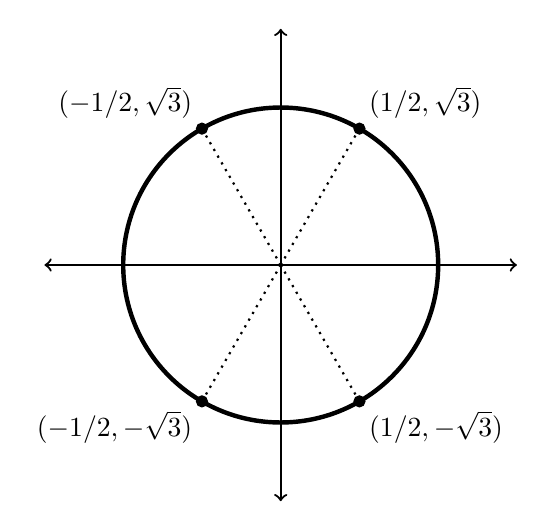
\begin{tikzpicture}[scale=2]
		% axes
		\draw [<->,thick] (0,1.5) -- (0,0) -- (1.5,0);
		\draw [<->,thick] (0,-1.5) -- (0,0) -- (-1.5,0);

		% unit circle
		\draw [ultra thick] (0,0) circle [radius=1];

		% points
		\draw [fill] (0.5,0.866) circle [radius=1pt];
		\draw [dotted,thick] (0,0) -- (0.5,0.866);
		\node [above right] at (0.5,0.866) {\( (1/2, \sqrt{3}) \)};

		\draw [fill] (-0.5,0.866) circle [radius=1pt];
		\draw [dotted,thick] (0,0) -- (-0.5,0.866);
		\node [above left] at (-0.5,0.866) {\( (-1/2, \sqrt{3}) \)};

		\draw [fill] (0.5,-0.866) circle [radius=1pt];
		\draw [dotted,thick] (0,0) -- (0.5,-0.866);
		\node [below right] at (0.5,-0.866) {\( (1/2, -\sqrt{3}) \)};

		\draw [fill] (-0.5,-0.866) circle [radius=1pt];
		\draw [dotted,thick] (0,0) -- (-0.5,-0.866);
		\node [below left] at (-0.5,-0.866) {\( (-1/2, -\sqrt{3}) \)};

	\end{tikzpicture}
\end{center}
Since multiplication of two complex numbers adds their angles and multiplies
their magnitudes, it is easy to see that the equation holds.
\done

\section*{Section 1.2}


\end{document}
